\chapter{Data Science Toolbox}

\href{https://www.coursera.org/course/datascitoolbox}{Coursera} classes, Feb 3rd - Mar 8th 2015. 
Examples of Data Science (DS) problems are:
\begin{itemize}
\item descriptive: simply describe data, like population census, no generalization is possible;
\item exploratory: look for connections and correlations in data, but {\it correlation does not imply causation}!;
\item inferential: extrapolate information from small sample to large population;
\item predictive: use data on one object to predict effect on another object ({\it prediction is very hard especially about the future!});
\item causal: identify causal relationships between variables (changes on one variable caused by changes on another variable);
\item mechanistic: find exact changes in variables leading to changes in another variable.
\end{itemize}

Confounding variable:

%\section{Statistical data science}



\section{R}

To start:
\begin{itemize}
\item \url{http://www.r-project.org/}: official page for \texttt{R}
\item \url{http://www.rstudio.com/}: according to many one of the best IDE\dots will see!
\item \href{http://cran.r-project.org/}{CRAN}: the Comprehensive R Archive Network, to look for packages
\item \href{http://www.bioconductor.org/}{Bioconductor Project}: packages for biological applications, wohoo!
\end{itemize}
Under CRAN Task Views packages related to various topics are grouped.
To install, load and see which functions are available in a package do:
\begin{lstlisting}[language=R]
install.packages(``pckgname'')
library(pckgname)
search()
\end{lstlisting}
To install packages from Bioconductor do:
\begin{lstlisting}[language=R]
source(``http://www.bioconductor.org/biocLite.R'')
biocLite()
biocLite(c(``pckg1'', ``pckg2'', ``pckg3''))
\end{lstlisting}

RmySQL

Building data products: R packages; rCharts; Shiny


\section{Git and GitHub}

To configure git with the github username and email:
\begin{lstlisting}[language=bash]
git config --global user.name asuccurro
git config --global user.email a.succurro@gmail.com
\end{lstlisting}
To avoid re-entering always user name and password in short time set a higher cache time:
\begin{lstlisting}[language=bash]
git config --global credential.helper 'cache --timeout=3600'
\end{lstlisting}
Whenever a ``new-repo'' is created, go to the chosen local \texttt{new-repo} and do:
\begin{lstlisting}[language=bash]
git init
git remote add origin https://github.com/asuccurro/new-repo.git
\end{lstlisting}
To add new files and commit and push to the remote github:
\begin{lstlisting}[language=bash]
git add stuff stuff morestuff
git commit -m 'message'
git push origin master
\end{lstlisting}
To commit all the modified files:
\begin{lstlisting}[language=bash]
git commit -am 'message'
\end{lstlisting}
Branching is used to modify a parallel version of the project. To switch to the branch called ``branchname'':
\begin{lstlisting}[language=bash]
git checkout -b branchname
\end{lstlisting}
To switch back to the master:
\begin{lstlisting}[language=bash]
git checkout master
\end{lstlisting}
To check where you are:
\begin{lstlisting}[language=bash]
git branch
\end{lstlisting}

\begin{lstlisting}[language=bash]
\end{lstlisting}

\begin{lstlisting}[language=bash]
\end{lstlisting}

\begin{lstlisting}[language=bash]
\end{lstlisting}

\begin{lstlisting}[language=bash]
\end{lstlisting}


To ``fork'' a project, go to the project github and click on the fork: this will simply copy the current version of the project
into the personal github. Then the copied project can be pulled:
\begin{lstlisting}[language=bash]
\end{lstlisting}



\begin{figure}[htb]\begin{center}
\subfigure[]{\label{fig:gitflow}
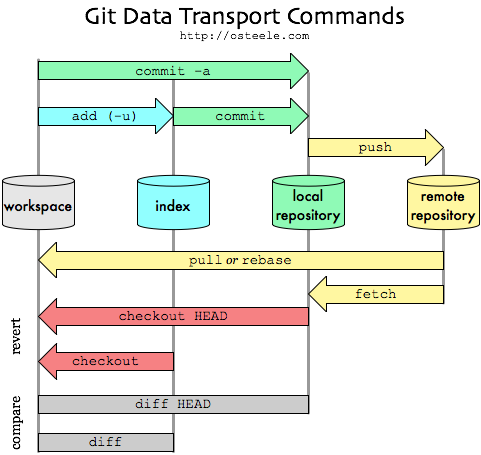
\includegraphics[width=0.5\textwidth]{00_datascientisttoolbox/pics/git-transport}}
\caption{From \href{http://gitready.com/beginner/2009/01/21/pushing-and-pulling.html}{gitready}.}
\end{center}\end{figure}


